% SSU Data Dash 2026: team report. Compile from this folder (Overleaf: upload the whole repository
% as a zip). Figures and dev_results.tex come from `python report/make_figures.py`; the final-check
% table from `python run.py validate && python run.py report` (run once, after the models are frozen).
% Keep the report to 4 pages, not counting the outside-data table and the appendix.
\documentclass[11pt]{article}
\usepackage[margin=2.2cm]{geometry}
\usepackage{graphicx,booktabs,hyperref,xcolor}
\graphicspath{{figures/}{../figures/}}
\setlength{\parskip}{4pt}
\newcommand{\todo}[1]{\textcolor{red}{[TODO: #1]}}

% Required: your team name and the full name of every team member.
\title{SSU Data Dash 2026: \todo{team name}}
\author{\todo{full names} Tiffany \todo{surname}, lanqi.qiu, steph.zheng, yuchen.ji}
\date{}

\begin{document}
\maketitle

\noindent\begin{tabular}{@{}ll}
\textbf{Video (YouTube, unlisted):} & \todo{https://youtu.be/...} \\
\textbf{Code and submission files (GitHub):} & \url{https://github.com/wsttiffanywu-oss/SSU-Data-Dash} \\
\end{tabular}

\section*{Summary}
We turned on the starter's gradient-boosted trees and fed them three kinds of information that a
valuer would have before a home is listed: the home itself, what its description says about its
condition, and what similar homes nearby sold for \emph{before} it was listed. Because the test homes
sell 0--4 months after our data ends, we validated every choice on six earlier months
(June--November 2025) predicted at gaps of 0, 1, 2 and 3 months, and trained the model on data that
was deliberately made just as stale. On those months the off-market median error (MdAPE) is
9.35\% against 18.70\% for the pass line, and list-aware is 4.24\% against 7.09\% for the list price.
Our 80\% prediction intervals covered 79.4--79.5\% of held-out off-market sales. The main lesson:
how stale the market data is matters as much as which features we use.

\section{Data and features}
We use only the competition files; no outside data. Every aggregate is computed from sales that
closed strictly before the home's listing date, for training rows as well as for the homes we
predict (unit tests check that a home's features never change when its own or any later sale
changes). \texttt{date\_sold}, \texttt{days\_on\_market} and the third-party estimate are not used: the
test files do not have them, and 70\% of the estimates are dated after the sale.

\textbf{Property.} Floor area (the middle of ranges such as ``1200--1399'', plus a flag for ranges),
bedrooms, bathrooms, parking, garage, lot front/depth/area (empty for condos), property type and
style, municipality, coordinates, months since 2021 and calendar month of listing.

\textbf{Remarks.} Eight hand-built phrase groups, chosen by reading which words go with prices above
or below the neighbourhood average in sales \emph{before} the dev months: renovated, luxury finishes,
new systems (roof, furnace), finished basement, landscaped, dated, major repairs and motivated
seller, as 0/1 columns, plus a net condition score. On pre-dev sales the score is monotonic:
homes scored $-2$ sold 7\% below their neighbourhood's price per sq ft, homes scored $+3$ 9\% above.
No remark contains a price, so the list price cannot leak into the off-market model through text.

\textbf{Market level.} Mean log price per sq ft of past sales by community $\times$ type
(3/6/12 months), community, type and the whole city (1/3/12 months), with counts, momentum
(3 vs 12 months) and a naive estimate (neighbourhood price per sq ft $\times$ this home's size).

\textbf{List-aware only.} Past mean log(sold/list) by community $\times$ type, community, type and city,
and how the list price compares with the naive market estimate.

\section{Models}
Both tracks use scikit-learn's \texttt{HistGradientBoostingRegressor}.
\textbf{Off-market} learns log(price) with 1,500 trees (learning rate 0.03, 127 leaves, at least 50
sales per leaf). \textbf{List-aware} learns log(sold/list), so the model only has to predict the
discount or premium on a price the market already set, and multiplies back by the list price; it uses
the default 100 trees, as larger ones overfit this weaker signal (Figure~\ref{fig:ablation}).
Both weight a sale half as much for every year it is older than the newest one.

\textbf{Staleness.} Trees cannot extrapolate: a home listed in August 2026 looks to them like one listed
in May. Training homes, however, always had market data up to the day before listing, while test homes
have data that is 0--4 months old. We therefore give each training home a random cut-off 0--120 days
before its listing, compute its market features from sales before that cut-off only, and tell the
model how old its data is. The model learns from 2021--2025 how prices drift while data ages.
At prediction time the windows end on the last day of data.

\begin{figure}[t]
\centering
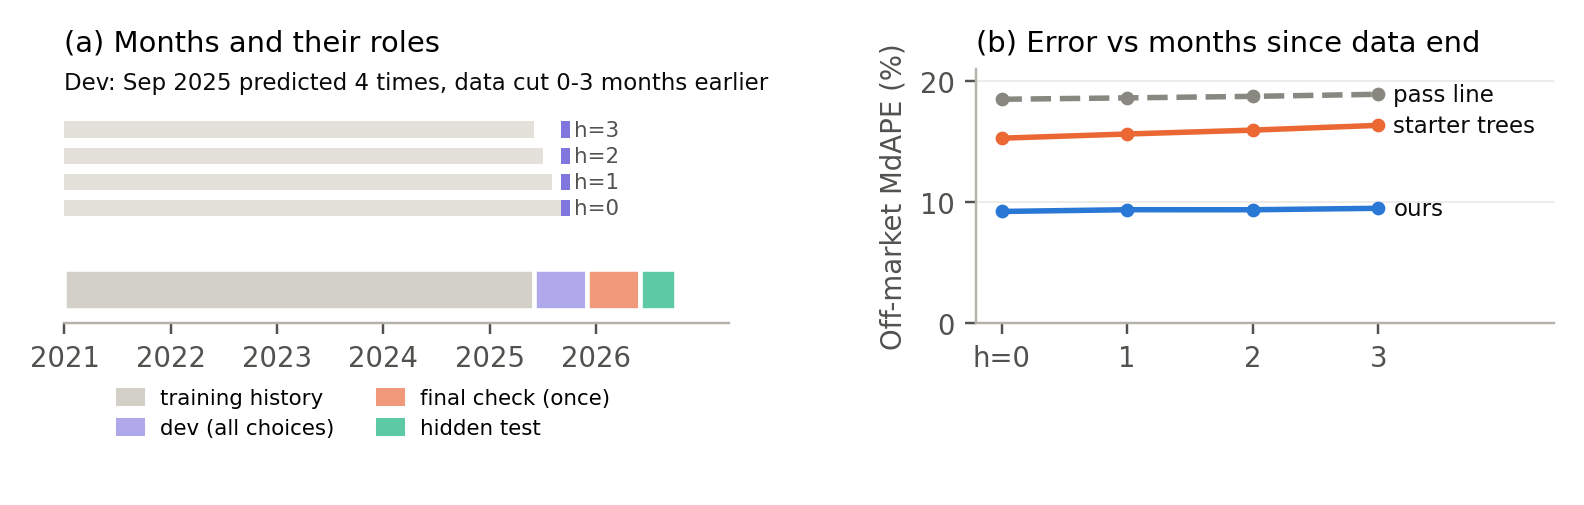
\includegraphics[width=\linewidth]{validation_design.png}
\caption{(a) Every choice was made on the dev months; the final check runs once. (b) Off-market dev
MdAPE when the data stops 0--3 months before the predicted month.}
\label{fig:design}
\end{figure}

\section{Validation}
Walk-forward only, never a random split. \textbf{Dev months} (June--November 2025): each month is
predicted four times, by models trained on sales closed before the month starts, or 1, 2 or 3 months
earlier (Figure~\ref{fig:design}a). This mirrors the test, where June is predicted from data ending
in May and September from data three months older. The official \texttt{run.py validate} only checks a
gap of 0, which flatters every model. All features, settings and the intervals were chosen on the
dev months (over 30 logged experiments in \texttt{experiments.md}).
\textbf{Final check} (December 2025--May 2026): run once, after freezing both models; we did not look
at it while developing \todo{run after freeze}.

\section{Results}
\begin{table}[h]
\centering\small
% Written by report/make_figures.py from outputs/dev_predictions_*.csv. Rerun instead of editing.
\begin{tabular}{llrrrrr}
\toprule
Track & Model & MdAPE & MAPE & Signed & MdAPE $h{=}0$ & MdAPE $h{=}3$ \\
\midrule
off-market & Pass line (community x type, 12 months) & 18.70 & 23.40 & +6.68 & 18.50 & 18.91 \\
off-market & Starter: 10 nearest earlier sales & 21.00 & 28.10 & +9.87 & 20.88 & 21.14 \\
off-market & \textbf{Ours} & 9.19 & 11.94 & +3.14 & 8.99 & 9.42 \\
\midrule
list-aware & Starter: list price & 7.09 & 7.92 & +5.82 & 7.09 & 7.09 \\
list-aware & \textbf{Ours} & 4.24 & 5.32 & +1.24 & 4.13 & 4.37 \\
\bottomrule
\end{tabular}

\caption{Dev months (12,169 homes, each predicted at gaps 0--3). Signed: median of
(predicted $-$ sold)/sold, above 0 means too high.}
\label{tab:dev}
\end{table}

\todo{Final check table: \texttt{python run.py validate \&\& python run.py report}, then
\texttt{\textbackslash input\{../reports/results\_table.tex\}} here, plus the same months at gaps 0--3.}

Both models clear their baselines by about half (Table~\ref{tab:dev}). Error barely grows with the gap
(off-market 9.21\% at $h{=}0$, 9.47\% at $h{=}3$; Figure~\ref{fig:design}b), which the staleness
training was meant to achieve. The largest gains came from past market levels ($-3.0$ points) and
larger trees ($-1.2$); Figure~\ref{fig:ablation} shows each step on its own.

\begin{figure}[t]
\centering
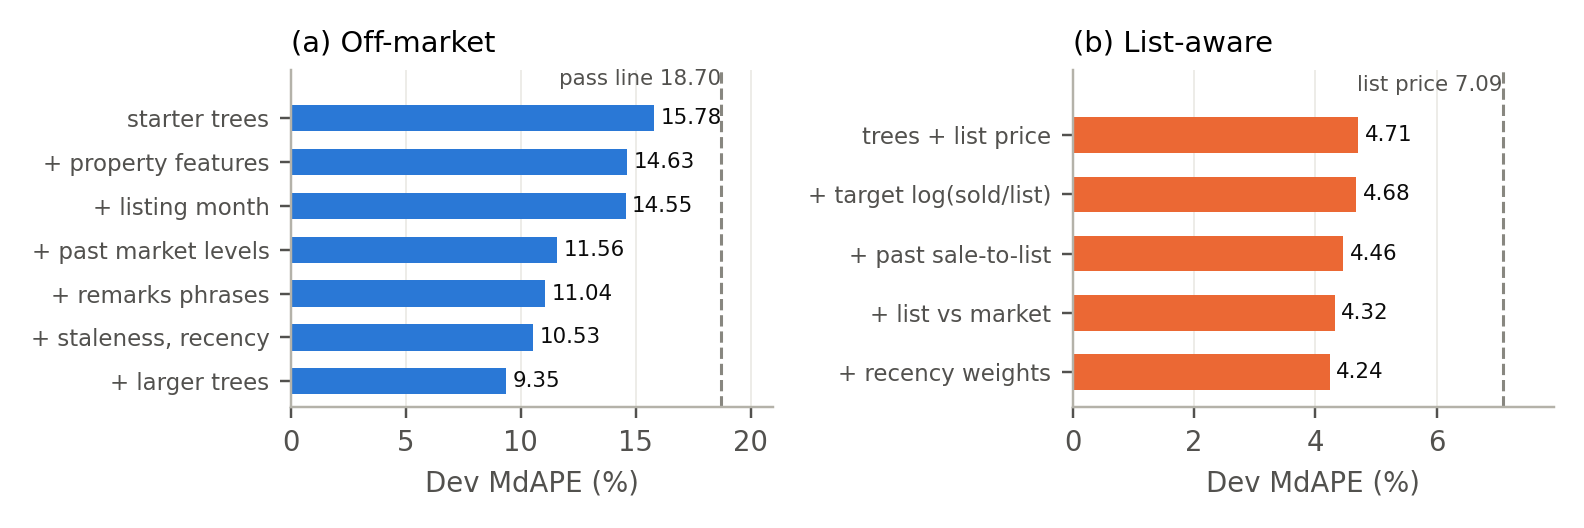
\includegraphics[width=\linewidth]{ablation.png}
\caption{Dev MdAPE as each idea is added on top of the previous ones.}
\label{fig:ablation}
\end{figure}

\textbf{Uncertainty.} An 80\% (90\%) interval is the prediction times the 10th and 90th (5th and 95th)
percentiles of past dev errors of homes of the same type and price third (split conformal).
Calibrated on three dev months and checked on the other three, both ways round, the off-market
80\% intervals covered 79.4\% and 79.5\% of sales (90\%: 89.9\%, 89.4\%), evenly across cheap, middle and
expensive homes (79.5/80.0/78.8\%) and gaps (79.3--79.6\%). Without price thirds the dearest homes
were covered only 72\%. List-aware coverage was 82.5\% and 76.2\%: it moves with the season (75--77\%
in June--August), so its intervals may be a little narrow for a summer test. Median 80\% widths are
35\% (off-market) and 16\% (list-aware) of the prediction; they are asymmetric because the models
still price slightly high. Intervals for every test home are in \texttt{outputs/}.

\section{Where the model fails}
\begin{figure}[t]
\centering
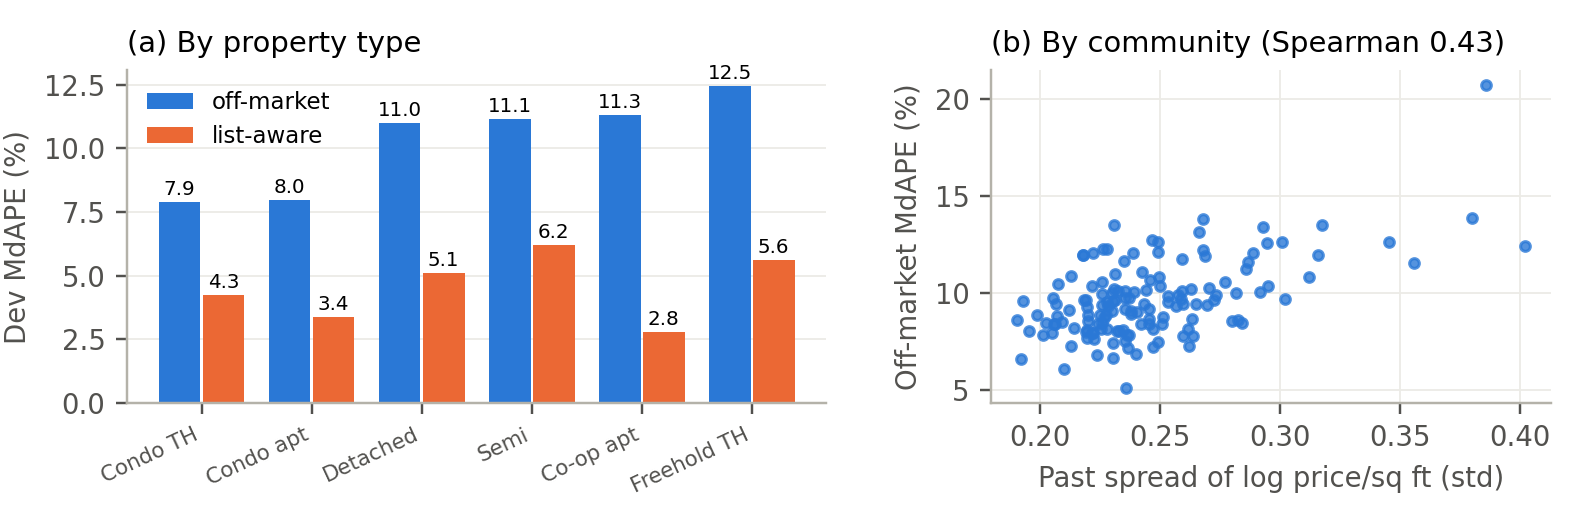
\includegraphics[width=\linewidth]{where_it_fails.png}
\caption{Dev MdAPE by property type, and off-market MdAPE by community against how spread out its
past prices per sq ft were (communities with at least 100 dev predictions).}
\label{fig:fails}
\end{figure}

\textbf{Freehold houses.} Condos are valued within 8\%; detached and semi-detached homes within 11\%,
freehold townhouses within 12.5\% (Figure~\ref{fig:fails}a). Houses differ in ways our columns do not
record (lot shape, renovation quality, the street).
\textbf{Mixed neighbourhoods.} A community's error tracks how spread out its past prices were
(Spearman 0.43), much more than how many sales it had ($-0.15$). The worst, Maplepark (20.7\%), has one
of the widest spreads (Figure~\ref{fig:fails}b).
\textbf{Expensive homes.} Off-market error rises from 7.5\% in the cheapest tenth of predictions to
13.5\% in the dearest. (By \emph{sold}-price decile the cheapest homes look overpriced by 10\% and the
dearest underpriced by 5\%; that is regression to the mean, not a bias of the model.)
\textbf{Not condition.} Error is flat across the remarks condition score (9.2--10.0\%), so the text
features handle condition.
\textbf{List-aware: unusual negotiations.} When a home sells between its list price and 10\% below,
the error is 2.5--3.3\%; bidding wars and deep discounts push it to 6.6--7.2\%. Nothing in a listing
predicts those.

\section{Limitations}
Both models still price high on the dev months (median signed error +2.8\% at $h{=}0$ to +4.3\% at
$h{=}3$ off-market, +0.9\% to +1.6\% list-aware), because prices kept falling through 2025.
We tried correcting this with the bias measured on the last 120 days of training data. On the dev months it
lowered MdAPE from 10.53\% to 10.38\% (tested before the final tuning), but at our final data end
(May 2026) it would raise every summer prediction by 3.4\%, a direction the dev months never tested,
right after a spring rebound and before the seasonal dip. We left it out.
The remarks features are hand-picked phrases; a text model might find more. We tried only
gradient-boosted trees. The intervals assume the next months' errors look like 2025's.

\section*{Outside data}
\begin{tabular}{lll}
\toprule
Source & URL & Periods covered \\
\midrule
None & & \\
\bottomrule
\end{tabular}

\section*{Reproducing our results}
From a fresh clone (Python 3.12, about 2 minutes; output is byte-identical on every run):\\
\texttt{python -m venv .venv \&\& .venv/bin/pip install -r requirements.txt}\\
\texttt{.venv/bin/python -m pytest -q}\\
\texttt{.venv/bin/python run.py predict \&\& .venv/bin/python run.py check}\\
Dev validation, intervals and figures: \texttt{python dev\_validate.py final},
\texttt{python phase3.py intervals}, \texttt{python phase3.py test}, \texttt{python report/make\_figures.py}.

\end{document}
